\chapter{Design and Implementation}
\label{chap:implementation}

Overview... Architecture... General Components

\section{Initial Situation}
Currently the data which should be analyzed is available through the protocols of the sessions of the national council. These protocols are publicly available and can be found at the website of the Austrian parliament (See \url{https://www.parlament.gv.at/PAKT/STPROT/}). They are in PDF-format and since the $20^{th}$ legislative period also available in HTML. As the extracting of the PDF-files would not result in sufficient quality, in this thesis only the data since the $20^{th}$ legislative period is being extracted and analyzed.

\subsection{Data Structure}
asdf

\section{Architecture}
Figure \ref{fig:general_architecture} shows the general architecture of the prototype which was implemented. The ETL-Application brings the data from the protocol in the database whereas the web server application shows statistics and graphs for the given data. The ETL-Application first reads an RSS feed which contains all the protocols for one legislative period. The retrieved HTML-files get parsed and are transformed into Java objects which get loaded into a relational database (in the prototype a PostgreSQL database was used). To visualize the then available data, the analysis engine queries the database and brings the data in a form which can be displayed (e.g. a graph structure). Furthermore, this data is made available via RESTful web services. The Polymer web application accesses these web services and shows the graphs and statistics. All the components will be described in more detailed in the later sections.

\begin{figure}
	\centering
	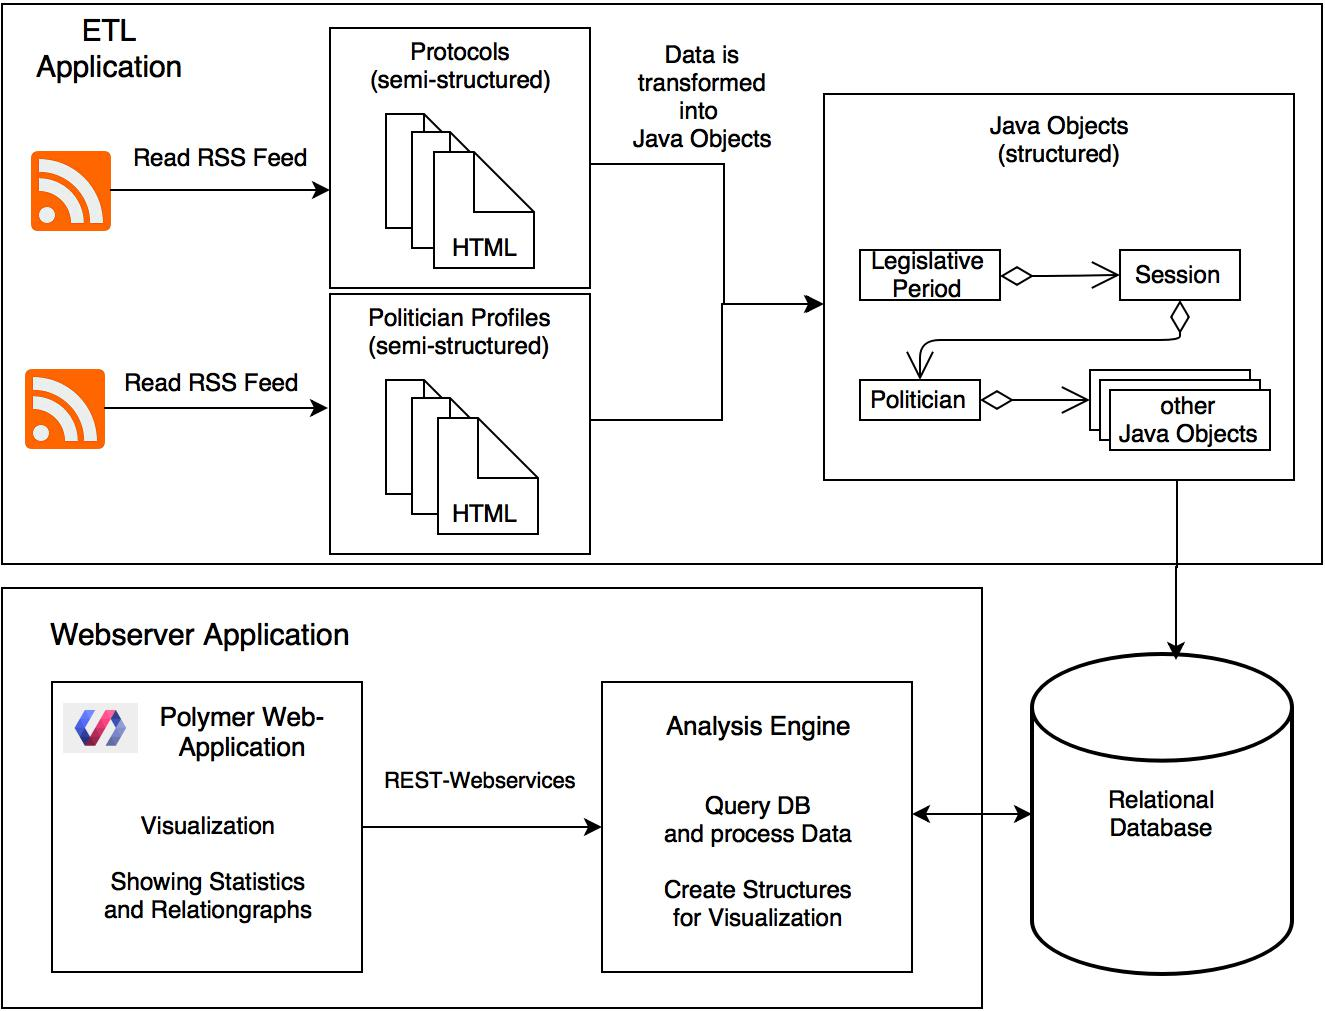
\includegraphics[width=\textwidth]{imgs/overall_architecture}
	\caption{General Architecture}
	\label{fig:general_architecture}
\end{figure}

\section{Data Extraction and Transforming}
\label{sec:data_extraction_transforming}

\section{Export into Database}
\label{sec:export_db}

\section{Analysis}
\label{sec:analysis}

\section{Visualization}
\label{sec:visualization}
